 % !TeX spellcheck = en_US
\documentclass[french]{yLectureNote}

\title{Optique Géométrique}
\subtitle{Niveau 1}
\author{Paulhenry Saux}
\date{\today}
\yLanguage{Français}

\professor{C.Gatel}%christophe.gatel@cemes.fr : section B sillon 7

\usepackage{graphicx}%----pour mettre des images
\usepackage[utf8]{inputenc}%---encodage
\usepackage{geometry}%---pour modifier les tailles et mettre a4paper
%\usepackage{awesomebox}%---pour les boites d'exercices, de pbq et de croquis ---d\'esactiv\'e pour les TP de PC
\usepackage{tikz}%---pour deiffner + d\'ependance de chemfig
\usepackage{tkz-tab}
\usepackage{chemfig}%---pour deiffner formules chimiques
\usepackage{chemformula}%---pour les formules chimiques en \'equation : \ch{...}
\usepackage{tabularx}%---pour dimensionner automatiquement les tableaux avec variable X
\usepackage{awesomebox}%---Pour les boites info, danger et autres
\usepackage{menukeys}%---Pour deiffner les touches de Calculatrice
\usepackage{fancyhdr}%---pour les en-t\^ete personnalis\'ees
\usepackage{blindtext}%---pour les liens
\usepackage{hyperref}%---pour les liens (\`a mettre en dernier)
\usepackage{caption}%---pour la francisation de la l\'egende table vers Tableau
\usepackage{pifont}
\usepackage{array}%---pour les tableaux
\usepackage{lipsum}
\usepackage{yFlatTable}
\usepackage{multicol}
\newcommand{\Lim}[1]{\lim\limits_{\substack{#1}}\:}
\renewcommand{\vec}{\overrightarrow}
\begin{document}
%\titleOne

\setcounter{chapter}{5}
\chapter{Oeil et instrument d'optiques}
\section{L'oeil}
\subsection{Constitution}
% La rétine est la couche de cellule photo-sensible qui comprend la fovéa, utilisée pour transformer l'information optique en information électrique, avec des connes et des batonnets.

% La lumière passe par l'humeur aqueuse, le cristallin et le corps vitré.

L'oeil est équivalent à un dioptre sphérique convexe et convergent. Quand l'indice du milieu se rapproche de celui de l'eoil, il devient moins convergent et on voit plis flou.

La focale image défini la position de la rétine. L'oeil modifie sa vergence en faisant varier $\bar{SC}$. En changeant la forme du cristallin, l'oeil fait la mise au point.

\begin{definition}[Accomodation]
Capacité de l'oeil à adapter la vergence du cristallin en fonction de la position de l'objet. La vergence évolue de $4\delta$. C'est l'amplitude de modification de la Vergence.
\end{definition}
\begin{definition}[Punctun proximum]
C'est la distance minimale de vision nette lorsque l'oeil accomode au maximum.
\end{definition}
\begin{definition}[Punctun remotum]
C'est la distance maximale de vision sans accomodation
\end{definition}
\begin{definition}[Oeil emmétrope]
Un oeil emmétrope est un oeil qui respecte les conditions de punctum proximum  de 25 cm et de punctum remotum à l'infini.
\end{definition}
\subsection{Défauts}
\begin{definition}[Myopie]
Le punctum remontum n'est plus l'infini. L'oeil est déjà trop convergent mais le punctum proximum se rapproche.
\end{definition}
\begin{definition}[Hypermetropie]
 L'oeil n'est pas assez convergent. Au bout d'un moment, l'oeil n'arrive plus à accomoder et l'oeil ne voit plus assez bien de près.
\end{definition}
\begin{definition}[Presbycie]
C'est la diminution de l'amplitude d'accomodation.
\end{definition}
\begin{definition}[Astigmatisme]
Il y  a un défaut de courbure de l'oeil qui crée une différence de focalisation, avec des points focaux multiples.
\end{definition}
\begin{definition}[Cataractacte]
le cristallin devient de plus en plus opaque.
\end{definition}
% \subsection{Limite de résolution}
% Elle est liée à la distance à laquelle on regarde. On parle donc d'angle et de limite de résolution angulaire.
% \subsection{Étude de cas de l'oeil myope}
% Le PP est inférieur à 25cm et le PR est à une distance finie pouvant aller à 1m.
%
% On met des lentilles divergentes pour corriger le problème.
%
% Le foyer image doit se trouver au PR, soit à 31-1=30 cm. donc avec une vergence de $-3,33\delta$.
\section{Caractéristiques d'un instrument d'optique}
\begin{definition}[Grandissement angulaire]
On définit le grandissement angulaire \(G_a = \frac{a_i}{a_o}\) avec les angles en fonction de la parallèle.
\end{definition}
L'instrument doit renvoyer un image à au moins 25cm de l'oeil.
\subsubsection{instruments subjectifs}
L'instrument doit fabriquer une image virtuelle car on regarde directemen dedans.

La première lentille doit etre convergente de petite focale.

Il a 2 parties : un système objectif (comme une lentille, toujours convergente, qui crée l'image) suivi d'un occulaire (qui sert à regarder l'image donnée par l'objectif).

L'occulaire récupère l'image formée par l'obejctif pour en former une à 25cm et jusqu'à l'infini\marginInfo{en l'agrandissant un peu, mais ce n'est pas son but premier}.

\subsubsection{Instruments objectifs}
Il sert à enregistrer une image pour l'afficher sur un écran. Il est composé seulement d'un système objectif.
\subsubsection{Généralités}
% Il sert à agrandir une image petite ou loin. Dans les 2 cas, on est en dessous de la limite de résolution de l'oeil et il faut augmenter le grandissement angulaire. Le but est donc d'augmenter les angles.
\criticalInfo{grossissement/Grandissement}{
On parle de grandissement quand on a une taille d'objet pas à l'infini. Quand l'image ou l'objet est à l'infini, on parle de grossissement (on raisonne uniquement avec les angles d'entrée ou de sortie)}
\begin{definition}[Puissance]
C'est l'angle de sortie sur la taille de l'objet : \(P = \frac{a'}{\bar{A_oB_o}}\).
\end{definition}
\subsection{Loupe}
\includegraphics[scale=0.5]{c1}

C'est une lentille convergente. On veut une image droite avec un objet réel. Il faut donc une image virtuelle. Il faut donc placer l'objet entre le centre optique et le foyer objet.
% On peut déplcer la loupe un peu quand elle est mise au point. L'oeil s'accomode alors.


\begin{theorem}[Caractéristiques pour une loupe]
Grossissement commercial pour $d_m$ : \(G = |\frac{a_i}{a}|\) avec \(a = \frac{A_oB_o}{d_m}\) et \(a_i = \frac{A_oB_o}{f_i}\). Donc \(G = \frac{d_m}{f_i}\)

Puissance \(P = \frac{1}{f_i} = V\)
\end{theorem}

\subsection{Microscope}
\includegraphics[scale=0.4]{c2}
\subsubsection{Fonctionnement}
On associe 2 lentilles convergentes : l'objectif est de faible focale (mm) et l'occulaire est de grande focale.
\begin{definition}[Intervalle optique $\Delta$]
la distance entre le foyer image de l'objectif et le foyer objet de l'occulaire.
\end{definition}

Comme la focale de l'objetcif est très faible, l'objet est situé après le foyer objet, donc une image réelle est produite, renversée. Il faut donc un occulaire pour produire une image à l'infini.
\begin{theorem}[Caractéristiques du microscope]
Puissance \(G_t(obj)P_{oc}\). Or, \(P_{oc} = \frac{1}{f_{i1}} = \frac{1}{f_{oc}}\) et \(G_t = \frac{\Delta}{f_{i2}} = \frac{\Delta}{f_{onj}}\) donc \(P = \frac{\Delta}{f_{obj}f_{oc}}\).

Grossissement commercial : \(G = G_{t,obj}G_{oc}\).
\end{theorem}

\section{Système afocal}
\subsection{Fonctionnement}
L'objet est très éloigné de façon à ce que les rayons sont parallèles et le fasecau émergent est parallèle. On souhaite donc augmenter l'angle de sortie et ainsi voir les détails\marginCritical{On parle de grossissement et non de grandissement car il n'y a plus de taille en jeu.}
\begin{definition}[Système afocal]
Un sysème afocal est un système ou le foyer image de la première lentille correspond au foyer objet de la deuxième lentielle. On en déduit que la vergence est nulle Ainsi, les rayons arrivent et ressortent parallèles entre eux.
\end{definition}

\subsection{Lunette astronomique}
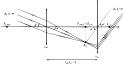
\includegraphics[scale=0.5]{lunette}

Le premier objectif est de grande distance focale et l'occulaire est de plus petite focale.

On fait correspondre le foyer image de l'objectif avec le foyer objet de l'occulaire.
\begin{theorem}[Caractéristiques]
 Grossissement  : \(G = |\frac{a_i}{a_o}|\) avec \(a_o = \frac{\bar{A_1B_1}}{\bar{O_1A_1}} = \frac{\bar{A_1B_1}}{f_{i1}}\) et \(a_i = \frac{\bar{A_1B_1}}{\bar{O_2A_1}} = -\frac{\bar{A_1B_1}}{f_{i2}}\). Donc \(G = |-\frac{f_{i1}}{f_{i2}}| = |\frac{f_{obj}}{f_{oc}}|\).%=|\frac{f_{obj}}{f_{oc}}|\).
\end{theorem}

\subsection{Lunette teresstre}
À la différence de la lunette astronomique, l'occulaire est divergent. La lunette tesrrestre nous permet d'obtenir une image droite

\end{document}

